\documentclass[border=20pt]{standalone}
\usepackage{tikz}
\usetikzlibrary{arrows.meta}
\usepackage{fontspec}
\setmainfont{Helvetica Neue}
\setsansfont{Helvetica Neue}

\begin{document}
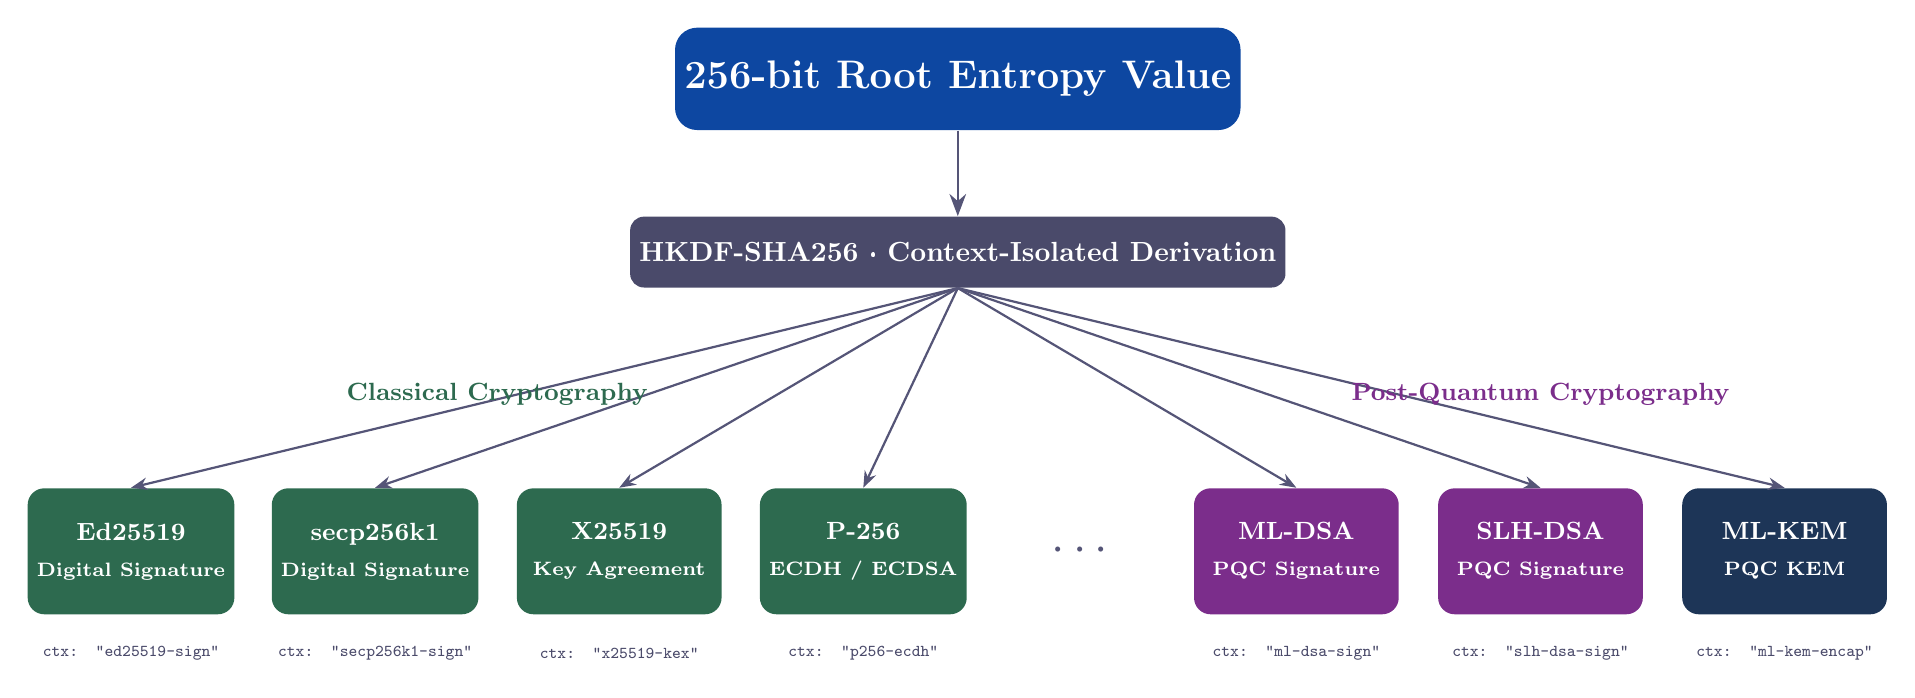
\begin{tikzpicture}[
    font=\sffamily,
    every node/.style={align=center},
]

% Colors
\definecolor{revcolor}{HTML}{0d47a1}
\definecolor{hkdfcolor}{HTML}{4a4a6a}
\definecolor{classicalcolor}{HTML}{2d6a4f}
\definecolor{pqsigcolor}{HTML}{7b2d8b}
\definecolor{pqkemcolor}{HTML}{1d3557}
\definecolor{linecolor}{HTML}{555577}

% Y coordinates
\def\revy{0}
\def\hkdfy{-2.2}
\def\boxy{-6.0}
\def\ctxy{-7.3}

% Box dimensions
\def\boxw{2.6}
\def\boxh{1.6}

% X positions
\def\xa{1.3}
\def\xb{4.4}
\def\xc{7.5}
\def\xd{10.6}
\def\xdots{13.35}
\def\xe{16.1}
\def\xf{19.2}
\def\xg{22.3}
\def\cx{11.8}

% REV node
\node[fill=revcolor, text=white, rounded corners=8pt,
    minimum width=5.5cm, minimum height=1.3cm,
    font=\Large\bfseries] (rev) at (\cx, \revy) {256-bit Root Entropy Value};

% HKDF node
\node[fill=hkdfcolor, text=white, rounded corners=5pt,
    minimum width=7.5cm, minimum height=0.9cm,
    font=\normalsize\bfseries] (hkdf) at (\cx, \hkdfy) {HKDF-SHA256 \textperiodcentered{} Context-Isolated Derivation};

% Arrow REV -> HKDF
\draw[-{Stealth[length=8pt]}, thick, color=linecolor] (rev.south) -- (hkdf.north);

% Algorithm boxes
\node[fill=classicalcolor, text=white, rounded corners=6pt,
    minimum width=\boxw cm, minimum height=\boxh cm,
    font=\small\bfseries] (ed25519) at (\xa, \boxy) {Ed25519\\[2pt]{\fontsize{7}{8}\selectfont Digital Signature}};

\node[fill=classicalcolor, text=white, rounded corners=6pt,
    minimum width=\boxw cm, minimum height=\boxh cm,
    font=\small\bfseries] (secp256k1) at (\xb, \boxy) {secp256k1\\[2pt]{\fontsize{7}{8}\selectfont Digital Signature}};

\node[fill=classicalcolor, text=white, rounded corners=6pt,
    minimum width=\boxw cm, minimum height=\boxh cm,
    font=\small\bfseries] (x25519) at (\xc, \boxy) {X25519\\[2pt]{\fontsize{7}{8}\selectfont Key Agreement}};

\node[fill=classicalcolor, text=white, rounded corners=6pt,
    minimum width=\boxw cm, minimum height=\boxh cm,
    font=\small\bfseries] (p256) at (\xd, \boxy) {P-256\\[2pt]{\fontsize{7}{8}\selectfont ECDH / ECDSA}};

\node[font=\LARGE\bfseries, text=linecolor] at (\xdots, \boxy) {$\cdots$};

\node[fill=pqsigcolor, text=white, rounded corners=6pt,
    minimum width=\boxw cm, minimum height=\boxh cm,
    font=\small\bfseries] (mldsa) at (\xe, \boxy) {ML-DSA\\[2pt]{\fontsize{7}{8}\selectfont PQC Signature}};

\node[fill=pqsigcolor, text=white, rounded corners=6pt,
    minimum width=\boxw cm, minimum height=\boxh cm,
    font=\small\bfseries] (slhdsa) at (\xf, \boxy) {SLH-DSA\\[2pt]{\fontsize{7}{8}\selectfont PQC Signature}};

\node[fill=pqkemcolor, text=white, rounded corners=6pt,
    minimum width=\boxw cm, minimum height=\boxh cm,
    font=\small\bfseries] (mlkem) at (\xg, \boxy) {ML-KEM\\[2pt]{\fontsize{7}{8}\selectfont PQC KEM}};

% Diagonal arrows from HKDF to each box
\foreach \n in {ed25519, secp256k1, x25519, p256, mldsa, slhdsa, mlkem} {
    \draw[-{Stealth[length=6pt]}, thick, color=linecolor]
        (hkdf.south) -- (\n.north);
}

% Category labels between HKDF and boxes
\node[font=\small\bfseries, text=classicalcolor] at (5.95, -4.0) {Classical Cryptography};
\node[font=\small\bfseries, text=pqsigcolor] at (19.2, -4.0) {Post-Quantum Cryptography};

% Context labels below each box
\node[font=\fontsize{6}{7}\selectfont\ttfamily, text=hkdfcolor] at (\xa, \ctxy) {ctx: "ed25519-sign"};
\node[font=\fontsize{6}{7}\selectfont\ttfamily, text=hkdfcolor] at (\xb, \ctxy) {ctx: "secp256k1-sign"};
\node[font=\fontsize{6}{7}\selectfont\ttfamily, text=hkdfcolor] at (\xc, \ctxy) {ctx: "x25519-kex"};
\node[font=\fontsize{6}{7}\selectfont\ttfamily, text=hkdfcolor] at (\xd, \ctxy) {ctx: "p256-ecdh"};
\node[font=\fontsize{6}{7}\selectfont\ttfamily, text=hkdfcolor] at (\xe, \ctxy) {ctx: "ml-dsa-sign"};
\node[font=\fontsize{6}{7}\selectfont\ttfamily, text=hkdfcolor] at (\xf, \ctxy) {ctx: "slh-dsa-sign"};
\node[font=\fontsize{6}{7}\selectfont\ttfamily, text=hkdfcolor] at (\xg, \ctxy) {ctx: "ml-kem-encap"};

\end{tikzpicture}
\end{document}
